\documentclass{sigchi}


\CopyrightYear{2017}
\setcopyright{acmcopyright}
 %\setcopyright{rightsretained}
%\setcopyright{usgov}
%\setcopyright{usgovmixed}
%\setcopyright{cagov}
%\setcopyright{cagovmixed}
% DOI
\doi{http://dx.doi.org/10.475/123_4}
% ISBN
\isbn{123-4567-24-567/08/06}
%Conference
\conferenceinfo{CHI'17,}{May 06--11, 2017, Denver, CO, USA}
%Price
\acmPrice{\$15.00}

% Use this command to override the default ACM copyright statement
% (e.g., for preprints).  Consult the conference website for the
% camera-ready copyright statement.

%% HOW TO OVERRIDE THE DEFAULT COPYRIGHT STRIP --
%% Please note you need to make sure the copy for your specific
%% license is used here!
% \toappear{
% Permission to make digital or hard copies of all or part of this work
% for personal or classroom use is granted without fee provided that
% copies are not made or distributed for profit or commercial advantage
% and that copies bear this notice and the full citation on the first
% page. Copyrights for components of this work owned by others than ACM
% must be honored. Abstracting with credit is permitted. To copy
% otherwise, or republish, to post on servers or to redistribute to
% lists, requires prior specific permission and/or a fee. Request
% permissions from \href{mailto:Permissions@acm.org}{Permissions@acm.org}. \\
% \emph{CHI '16},  May 07--12, 2016, San Jose, CA, USA \\
% ACM xxx-x-xxxx-xxxx-x/xx/xx\ldots \$15.00 \\
% DOI: \url{http://dx.doi.org/xx.xxxx/xxxxxxx.xxxxxxx}
% }

% Arabic page numbers for submission.  Remove this line to eliminate
% page numbers for the camera ready copy
% \pagenumbering{arabic}

% Load basic packages
\usepackage{balance}       % to better equalize the last page
\usepackage{graphics}      % for EPS, load graphicx instead 
\usepackage[T1]{fontenc}   % for umlauts and other diaeresis
\usepackage{txfonts}
\usepackage{mathptmx}
\usepackage[pdflang={en-US},pdftex]{hyperref}
\usepackage{color}
\usepackage{booktabs}
\usepackage{textcomp}
\usepackage{soul}
\usepackage{enumitem}

% Some optional stuff you might like/need.
\usepackage{microtype}        % Improved Tracking and Kerning
% \usepackage[all]{hypcap}    % Fixes bug in hyperref caption linking
\usepackage{ccicons}          % Cite your images correctly!
% \usepackage[utf8]{inputenc} % for a UTF8 editor only

% If you want to use todo notes, marginpars etc. during creation of
% your draft document, you have to enable the "chi_draft" option for
% the document class. To do this, change the very first line to:
% "\documentclass[chi_draft]{sigchi}". You can then place todo notes
% by using the "\todo{...}"  command. Make sure to disable the draft
% option again before submitting your final document.
\usepackage{todonotes}

% Paper metadata (use plain text, for PDF inclusion and later
% re-using, if desired).  Use \emtpyauthor when submitting for review
% so you remain anonymous.
\def\plaintitle{Someone to Read with: Design of and Experiences with \\ an In-Home Learning Companion Robot for Reading}
\def\plainauthor{}
\def\emptyauthor{}
\def\plainkeywords{Human-robot interaction; interest development; reading education; educational robots; design probes}
\def\plaingeneralterms{Documentation, Standardization}

% llt: Define a global style for URLs, rather that the default one
\makeatletter
\def\url@leostyle{%
  \@ifundefined{selectfont}{
    \def\UrlFont{\sf}
  }{
    \def\UrlFont{\small\bf\ttfamily}
  }}
\makeatother
\urlstyle{leo}

% To make various LaTeX processors do the right thing with page size.
\def\pprw{8.5in}
\def\pprh{11in}
\special{papersize=\pprw,\pprh}
\setlength{\paperwidth}{\pprw}
\setlength{\paperheight}{\pprh}
\setlength{\pdfpagewidth}{\pprw}
\setlength{\pdfpageheight}{\pprh}

% Make sure hyperref comes last of your loaded packages, to give it a
% fighting chance of not being over-written, since its job is to
% redefine many LaTeX commands.
\definecolor{linkColor}{RGB}{6,125,233}
\hypersetup{%
  pdftitle={\plaintitle},
% Use \plainauthor for final version.
  pdfauthor={\plainauthor},
%  pdfauthor={\emptyauthor},
  pdfkeywords={\plainkeywords},
  pdfdisplaydoctitle=true, % For Accessibility
  bookmarksnumbered,
  pdfstartview={FitH},
  colorlinks,
  citecolor=black,
  filecolor=black,
  linkcolor=black,
  urlcolor=linkColor,
  breaklinks=true,
  hypertexnames=false
}

% create a shortcut to typeset table headings
% \newcommand\tabhead[1]{\small\textbf{#1}}

% End of preamble. Here it comes the document.
\begin{document}

\title{\plaintitle\vspace{56pt}}

%\numberofauthors{2}
%\author{%
%  \alignauthor{Leave Authors Anonymous\\
%    \affaddr{for Submission}\\
%    \affaddr{City, Country}\\
%    \email{e-mail address}}\\
%  \alignauthor{Leave Authors Anonymous\\
%    \affaddr{for Submission}\\
%    \affaddr{City, Country}\\
%    \email{e-mail address}}\\
%  %\alignauthor{Leave Authors Anonymous\\
%   % \affaddr{for Submission}\\
%    %\affaddr{City, Country}\\
%    %\email{e-mail address}}\\
%}

\maketitle

\begin{abstract}
  The development of literacy and reading proficiency is a building block of lifelong learning that must be supported both in the classroom and at home. While the promise of interactive learning technologies has widely been demonstrated, little is known about how an interactive robot might play a role in this development. We used eight design features based on recommendations from interest-development and human-robot-interaction literatures to design an in-home learning companion robot for children aged 11--12. The robot was used as a technology probe to explore families' ($N=8$) habits and views about reading, how a reading technology might be used, and how children perceived reading with the robot. Our results indicate reading with the learning companion to be a way to socially engage with reading, which may promote the development of reading interest and ability. We discuss design and research implications based on our findings.
  %145 words, 150 max
\end{abstract}

\category{H.1.2.}{\textbf{Models and Principles}}{User/Machine Systems}{\textit{---human factors, software psychology}}
\category{H.5.2.}{\textbf{Information Interfaces and Presentation}}{User Interfaces}{\textit{---evaluation/methodology, user-centered design}}

\keywords{\plainkeywords}

\section{Introduction}

\begin{figure}[t]
	\centering
	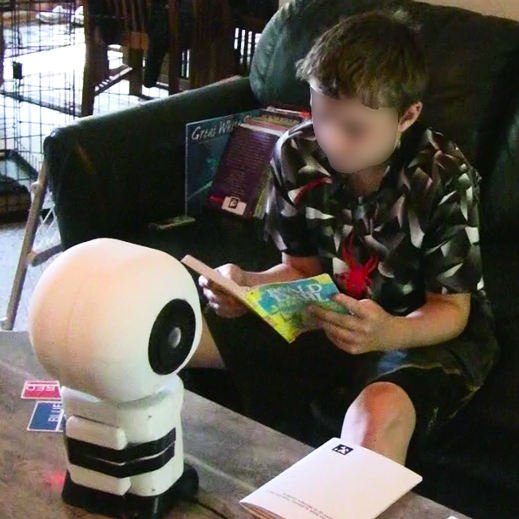
\includegraphics[width=1\columnwidth]{figures/childWithRobotTeaser_2}
	\caption{A study participant reads James and the Giant Peach to Minnie, our learning companion robot.}~\label{fig:teaser}\vspace{-16pt}
\end{figure}

Reading has long had an important and established place in education, and developing literacy and reading proficiency is considered a basic and essential element of learning \cite{McCormick:1994,Freire:1983}. While classroom instruction for younger readers is an important part of this process, practicing and engaging with reading at home is also crucial for these students \cite{Baker:1997}. With drastic technological advances in the last decade, using robots as educational agents to support learning both in classrooms and in the home has become increasingly viable \cite{Benitti:2012}. These educational robots can act as learning companions, tutors, or instructional agents, providing individually tailored instruction to children \cite{Miller:2008}. When used in the home, robots promise to support student learning and skill-building to supplement classroom instruction.

One type of instructional support that has proven beneficial to both learning outcomes and student engagement is the development of \textit{interest} in a domain \cite{Hidi:2006}, and supporting this development can be particularly useful for young readers \cite{Jones:2011}. However, little is known about how an in-home learning companion robot might provide students with support for interest and engagement in reading. In this paper, we present work aimed to explore how young readers currently engage in reading at home and how they imagine technologies such as robots could enhance this activity; to observe how they interact with a robot designed as an in-home learning companion for reading; and to explore their beliefs about how they might use and benefit from a robot as a learning companion. To pursue these goals, we developed an in-home learning companion robot, named ``Minnie,'' to use as a technology probe \cite{Hutchinson:2003}.
% The name Minnie is after the Owl of the Roman Goddess Minerva.

In the following sections, we report on the use of Minnie, a robot designed with guidelines offered by prior research in interest development and human-robot interaction, as a probe to gain a better understanding of how a learning companion robot may be used in a child's home, and how our design features will be perceived by the child and their family. After providing a brief background on the research that guided our work, we describe how the robot was developed and used as a technology probe. We then detail our data collection methods and results, discuss the implications of these results, and finally conclude with theoretical and practical contributions to both interest development and human-robot interaction.

\section{Background}
Our work is inspired by prior research that has highlighted the educational promise of robots in the home and their role as social agents compared to other learning technologies. Han et al. \cite{Han:2005} were among the first to report on testing an educational robot for children in their homes. They found that a home robot promoted engagement, interest, and learning in English and that users considered the robot to be friendlier than other learning media. These benefits may be due to the robot's ability to better connect socially with its user and perform more appropriate behavioral strategies than other computerized agents \cite{Brown:2013}, as social interactions between humans have been found to positively influence interest and learning in a task \cite{Sansone:2005}. Other studies in human-robot interaction have found robots to be more engaging and life-like \cite{Kiesler:2008}; appealing, perceptive and helpful \cite{Wainer:2007}; and positive and natural \cite{Bainbridge:2011} than other computerized agents. This social nature of human-robot interaction motivates our exploration of robots as learning companions rather than other computerized agents or alternative learning technologies for reading.

Our investigation draws on research in interest development as well as in human-robot interaction to identify guidelines for supporting student engagement and interest in a reading task. Interest-development researchers distinguish between \textit{situational interest}, a psychological state characterized by increased focus and attention, and \textit{individual interest}, a predisposition to reengage with specific content \cite{Krapp:1999}. The Four-phase Model of Interest Development proposed by Hidi and Renninger \cite{Hidi:2006} further refines the situational-individual interest distinction into four progressive phases of interest: Triggered Situational, Maintained Situational, Emerging Individual, and Well-Developed Individual. The phases of the Four-phase Model are considered to be sequential and distinct, with each subsequent phase building off the previous. Interest, in this model, is characterized as increasing positive affect, value, and knowledge for the domain \cite{Renninger:2011}.

Promoting situational interest by successfully \textit{triggering} (or catching) and then \textit{maintaining} (or holding) a student's interest during successive interactions can promote the development and maintenance of individual interest \cite{Hidi:2006, Mitchell:1993}. Guidelines for catching and holding interest from this area of research include providing students with autonomy in choosing educational materials \cite{Jones:2011}; setting and monitoring reading goals \cite{Cabral:2015}; providing materials that align with student topic interests \cite{Ainley:2002} and that students believe they have the ability to be successful with; providing social partners who demonstrate interest in the activity \cite{Sansone:2005}; and reading out-loud to a social partner \cite{Rasinski:2003}. 

Findings from human-robot interaction studies also provide several guidelines for increasing user engagement in human-robot interaction, including the robot establishing and maintaining direct eye contact when speaking to its user \cite{Mutlu:2011}; providing tailored recommendations for content \cite{Lim:2013}; expressing empathy \cite{Leite:2012}; and making reference to previous interactions \cite{Leite:2009}. By utilizing these design guidelines, we believe a robotic agent may be a powerful tool for supporting interest and engagement in reading for young readers. Several specific features can be incorporated into a learning companion robot in order to promote student interest and engagement in reading. The next section details how the design process for our technology probe integrates these features.

% TODO: Making this text into a Background section is one of the biggest changes I made, which the readers will expect to see. As a background section, it could be extended a little bit to make sure that you are covering your bases on other related work from HRI, CHI, etc. so that if one of your reviewers did or know work that's similar, they don't go ballistic on us for having missed it.

% NOTE: I thought about adding a few citations about promoting social interaction though the physical design.  Duffy, 2003: Anthropomorphism and the social robot http://dx.doi.org/10.1016/S0921-8890(02)00374-3 ; and Tung, 2016: Child Perception of Humanoid Robot Appearance and Behavior doi: 10.1080/10447318.2016.1172808.  Martini 2015: Minimal physical features required for social robots. My hesitation is that we are sort of locked into only having 8 design features, since that is in our abstract.  Thoughts?

%Added some Interest development theory to support classifying the children using the four-phase model terminology.

\section{DESIGN OF THE TECHNOLOGY PROBE}
 For this study, we first developed a learning companion robot, Minnie, based on the design guidelines discussed in the previous section. Following design research practices from prior work, such as work by Odom et. al \cite{Odom:2012}, we then conducted short in-home visits with families to use the learning companion robot as a \textit{technology probe} \cite{Hutchinson:2003} for discussion and reflection on how a reading technology might impact current reading habits in each home. Hutchinson et al. \cite{Hutchinson:2003} describe the technology probe approach as a method with three goals---understanding the user's needs and feelings about the technology, field-testing a technology, and reflection on new possibilities for the technology---that reflect our aims for this study. At this stage of development, our prior understanding of the intended user may not be sufficient, which may limit our view of how and what the learning companion robot should do. The introduction of the learning companion into the home may uncover unknown user needs and expectations as well as inspire new thoughts on and possibilities for the learning companion's use. We intend to explore these ideas to inform design modifications to the learning companion robot prior to empirical testing. Thus, our field testing of the robot is conducted concurrent to deep exploration of the design space through the eyes of the user. In essence, we must study the user, the technology, and their interaction all at the same time.

% TODO: This last sentence is great, and you explain what you mean by it in the second half of the next paragraph, but perhaps make it a bit more clear?
% DONE: Added one more sentence for clarity.
 
 We began the in-home visit by asking one child (referred to after as the \textit{main child}) to complete a short survey on individual interest in reading, followed by an interview (pre-) with the family. After the pre-interview, we introduced our learning companion robot to the family and asked the main child in the home to interact with it for a short period of time (approximately 30 minutes). Following the interaction, we asked the main child to complete another short survey, this time about their situational interest during the interaction. Finally, we completed a second interview (post-) with the family. In the spirit of using the technology as a probe, we did not limit the discussion or interaction with the robot to our preconceived ideas about how, when and where the learning companion should and would be used. Rather, we allowed families to explore ideas about how they would like to or would use this or another technology for reading. The following paragraphs describe this data collection method and subsequent analytic approach in more detail.
 
\subsection{Development of the Robot Platform}
Our initial design of the learning companion robot was guided by a desire to leverage the power of social interaction to promote interest and engagement in reading. We determined that a small, desktop humanoid robot with multiple methods of interaction and non-verbal expression would be appropriate for interaction with a child over the activity of reading. We also felt that the robot should be built on a simple, modifiable, and inexpensive platform in order to model the type of constraints inherent in an affordable commercially available robot. This intuition led us to create the robot using a modified version of a freely available 3D-printable robot design from Hello Robo\footnote{Hello Robo: \href{http://www.hello-robo.com/}{http://www.hello-robo.com/}} called Maki. A more expensive pre-made robot such as the popular Nao platform by SoftBank Robotics,\footnote{SoftBank Robotics: \href{https://www.ald.softbankrobotics.com/en}{https://www.ald.softbankrobotics.com/en}} while possibly offering a more reliable and polished experience, is not flexible in its physical and hardware design, and the cost would preclude many families from actual use in the their homes. The original robot from Hello Robo stands 13.5 inches and has a static torso without any movable appendages (see Figure \ref{fig:complete-system}). The head and neck of the robot contain five servo controlled motions, including two closing eyelids, a pair of eyes that move laterally together, and vertical and horizontal head movements. These motion options allowed us to create specific robot behaviors to provide a life-like feel (e.g., blinking eyes) and non-verbal communication (e.g., looking directly at the child). 

To perform the necessary computation and facilitate human-robot communication, we modified the original robot design by Hello Robo by adding four pieces of hardware to the robot. First, we integrated a Raspberry Pi 3 Model B\footnote{Raspberry Pi: \href{https://www.raspberrypi.org/}{https://www.raspberrypi.org/}} microcomputer running the Debian 7 operating system\footnote{Debian: \href{https://www.debian.org}{https://www.debian.org}} to perform the sensing, actuation, and computation necessary for the robot's functioning and interaction with the child. Integration of the microcomputer also required us to modify the 3D model of the robot, and thus we extended the back wall of the robot's torso in the shape of a small ``backpack'' that would house the computer and provide us or the end users with easy access to the hardware. Second, we embedded a speaker in each of the ear pieces to allow the robot to utilize text-to-speech responses to the child. Third, we included an RFID reader in the lower front of the robot to allow the child to respond to the robot with four color coded, pre-programmed RFID cards. Roughly, the cards allowed the child to \textit{say} ``yes/continue,'' ``no/stop,'' ``pause,'' and ``repeat'' to the robot. Fourth, we added a USB camera to achieve two purposes: allowing video input to process facial recognition, which we used for facial tracking and reading visual tags (AprilTags\footnote{AprilTags: \href{https://april.eecs.umich.edu/wiki/AprilTags}{https://april.eecs.umich.edu/wiki/AprilTags} }) placed within books. Each time an RFID card or an AprilTag is scanned, Minnie blinks and makes a distinct beep to let the child know that the scan was registered. The robot platform allows us to implement the eight design elements we identified from our literature review.

\begin{figure}
	\centering
	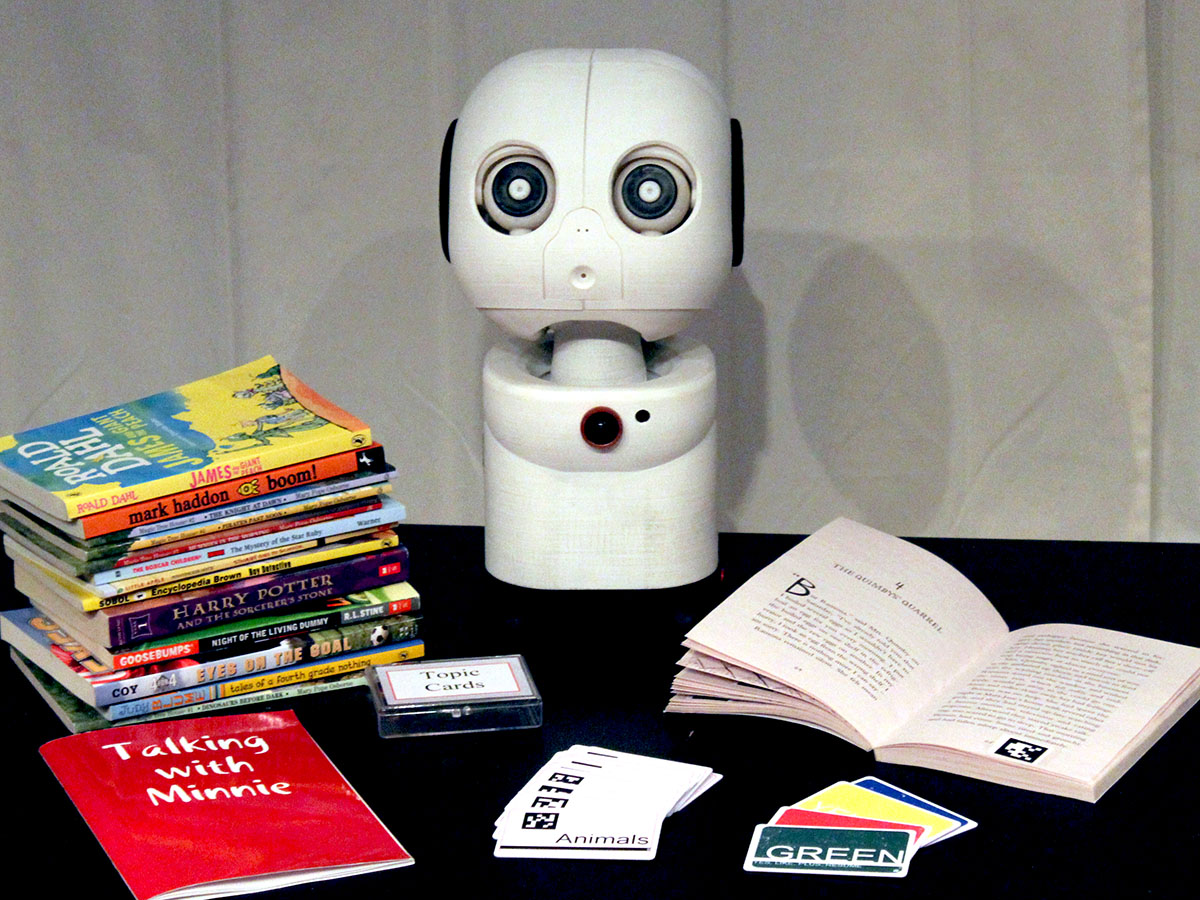
\includegraphics[width=\columnwidth]{figures/Complete-Minnie-System.jpg}
	\caption{Image of the learning companion robot, Minnie, used in the study as well as the introductory ``Talking with Minnie'' book, RFID topic and interaction cards, and books augmented with AR tags. The robot's camera is the red circle on the upper torso. The RFID reader is below the camera, and indicated by a red light when the robot is on. }~\label{fig:complete-system}\vspace{-16pt}
\end{figure}

\subsection{Interaction Design of the Robot}

The interaction design of our technology probe utilizes the eight guidelines, identified from research in interest development and human-robot interaction to support student engagement and interest in reading, in the following design elements:

\begin{enumerate}[leftmargin=0ex,itemindent=5.25ex,itemsep=0.25ex]

\item[$DE1$] Providing students with autonomy in choosing educational materials;
\item[$DE2$] Setting and monitoring reading goals;
\item[$DE3$] Providing materials that align with student topic interests and with which students believe they have the ability to be successful;
\item[$DE4$] Providing a social partner that indicate interest in the reading activity;
\item[$DE5$] Reading out-loud to a social partner;
\item[$DE6$] Having the robot maintain eye contact when speaking;
\item[$DE7$] Providing tailored recommendations for content;
\item[$DE8$] Making references to previous interactions. 
\end{enumerate}


 In the description of the interaction design of the robot below, we will identify where design features are addressed in parentheses. We begin with a discussion of the general design of the robot interaction, followed by specific interaction details particular to this study.
% TODO: One of the questions the readers are going to have is where these guidelines come from specifically. After reading the rest of the design section, it is probably best to integrate that information here where you list the design features.
% DONE: Tried to clarify.  See NOTE below.
% NOTE: Not sure what you mean here?  These exact guidelines are layed out in the background section, and are repeated here and organized as a list for clarity.  Perhaps that is what is not clear.  So, I reworded the first sentence in the paragraph above.  Hopefully, that helps.

\subsubsection{Design of the Interaction Flow}

During the interaction, Minnie, the learning companion robot, uses face recognition to track the child's position and turn its head and eyes toward the child to establish eye contact (\textit{DE}6). However, to prevent long durations of eye contact from eliciting discomfort, the robot makes idle head and eye movements and engages in gaze aversion, and the robot also continually uses pre-scripted dialog based on an interaction flow, described below, which we developed through iterative design and testing.

\textit{Introduction --} The interaction flow begins with Minnie saying ``hello'' to the child and providing a brief backstory on why the robot is there (i.e., the robot tells the child that she is a reading coach in training). The child is then instructed to scan and read a book, ``Talking with Minnie,'' that was written by the authors of this work, and is used to teach the child how to interact with the robot. This book is written as a story, but the content guides the child through the use of each interactive tool (e.g., how to scan the RFID cards and AprilTags as well as, and they mean), and how to work with Minnie (e.g., read out loud and scan AprilTags). The robot then asks the child to complete a topic-sort activity using 10 topic interest cards (e.g., mystery, art, science, and/or sci-fi/fantasy) with AprilTags. For this activity, Minnie the child to scan the topics they like, followed by any topics they do not like. The robot stores this ion in the user profile for the child and later uses this as part of a book suggestion algorithm. Figure \ref{fig:introduction} show2 illustrates a child working during the introduction process.

\begin{figure}
	\centering
	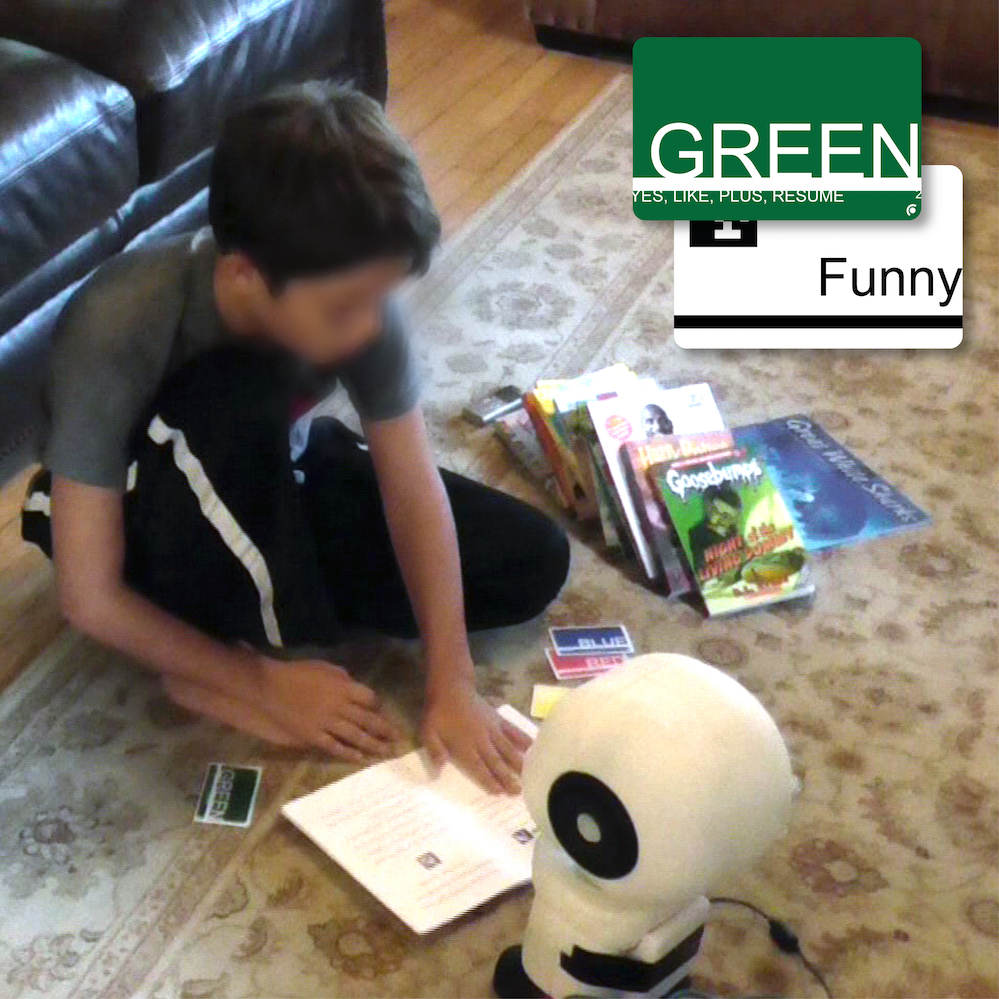
\includegraphics[width=1\columnwidth]{figures/Child-with-Minnie}
	\caption{Image of a child working with Minnie during the introductory process. The child is holding a topic interest card, and has placed the Talking with Minnie book on the floor in front of Minnie. The books available for the child to read appear on the right of the image. An example of a green RFID card and a topic interest card with an April tag are superimposed on the top right of the figure.}
	\label{fig:introduction}
\end{figure}

\textit{Goal Setting --} After completing the initial introduction phase, Minnie begins the process of setting reading goals and selecting books. During this process, Minnie informs the child of a goal for reading time that day (\textit{DE}2)---for this study, standardized at 20 minutes in length---before each reading session, and begins tracking the time spent reading after a book is chosen. The learning companion robot will then check the user profile for a book, a previously read book that has not been finished. If a current book exists, Minnie will remind the child of what they were last reading and the page number they were on (\textit{DE}8). The child then has the option to continue or not. If the is no current book selection, Minnie suggests three books (out of a set of the 16 available) to the child that the child may be interested in reading.

The robot's suggestions for books are based on an selection method that uses the child's reading ability, interest in reading, usual time spent reading, and topic interests to recommend page length, reading level, and topical content of a book for the child (\textit{DE}3).  Books are first filtered based on reading ability and interest in reading, to include books at an appropriate reading level \textit{(DE3)}. We then use the child's average reading time to filter the books based on length (i.e. longer books for children who read for a longer duration).  Finally, the program then assigns each book listed in the library a score based on the how well they match the topic interests of the child, and creates a priority cue with the highest scoring book at the front of the cue. The top three books in the priority cue are offered to the child as suggested titles (\textit{DE}7). The child may chose any book they wish (\textit{DE}1), and scan the AprilTag placed on the back of the book they choose to indicate their selection. The robot then updates the user profile to store the selected book as the child's current book;, Minnie confirms the title of the book with the child;, and the child is asked to begin reading on page one, which marks the beginning of the reading phase.
% TODO: The reader will want to know how this "algorithm" works to come up with the recommendation. Is it some kind of cost-based search?
% DONE: I hope, see note below.  Changed to describing this as a selectoin "method" using a series of filters.
% NOTE: It is not that sophisticated really, and maybe calling it an algorithm is misleading.  I added some more detail, but to explain it further will take a lot more space, so hopefully this is sufficient.  If the lexile score for the child is known we enter that into the user profile.  If not. we use Lexile estimates of a range of scores for each grade level.  If the child is described as reading at grade level we use the middle score, if they are above we use the lower limit and below we use the lower limit.  Once the user lexile is set, we add or subtract points based on their reading intereest (using our survey we set five levels of adjustments).  Theeeen, we look for books that are +/- 100 the adjusted lexile score.  The next filter figures that we would want kids to read about one book per week and we guess about 1 minute per page (book difficulty is already adjust for), so we do a quick calculation of idealPageLength = bookLength * time per page / readingTimePerDay * 7 (days in the week) .  This is definitely a back of the napkin formula.  

\textit{Reading --} In the reading phase, the child is asked to read \textit{out loud} to Minnie (\textit{DE}5). Minnie is designed to make semi-randomized movements during the reading phase, which include blinking, moving its eyes, and small turns of its head in order to appear engaged in the reading (\textit{DE}4). As the child reads, AprilTags will appear roughly every three to six pages of each book, and the child is instructed to scan these tags when they encounter them. The tag ID is linked to a specific comment, written by our research team, related to what is currently happening in the book (\textit{DE}4). When a scan is received by Minnie, it blinks, makes a distinct \textit{beep}, and delivers the comment via text-to-speech. Each time a book tag is scanned, the user profile is updated to store that page as the current page. During the reading phase, the child may continue to read, scan the \textit{yellow} RFID to pause reading, or scan the \textit{red} RFID to quit reading. This phase continues until the child chooses to quit, or scans the last age of the book. At that point, Minnie enters the ``end- reading'' phase.


\textit{End Reading --} The end of the reading phase is triggered by either the child choosing to quit reading or when a book has been completed. In both cases, Minnie will compare the time spent reading to the reading goal previously set (\textit{DE}2). If the child have met the reading goal for the day, Minnie will congratulate the child, and begin the shut-down process. Shutting down consists of thanking the child for the time spent reading, encouraging them to read more the next day, and telling the child that the learning companion robot is going to sleep. If the reading goal has not been met, the robot will let the child know how much time is remaining to reach the goal and ask whether or not they should continue reading. If the child choses to continue reading, Minnie asks if the child would like to read the same book or a new one and then re-enters the reading phase. Otherwise, Minnie initiates the shut-down procedure. 

\textit{Updating User Profile --} When a child scans the last page of a book, Minnie will ask the child whether they liked the book. The child can respond with \textit{yes} (green card), \textit{no} (red card), or \textit{a little} (yellow card). This response is stored in the user profile and is used to trigger a recalculation of book suggestion scores. For books the child liked, the topics associated with that book will be given a higher score rating, which will move books with similar topics up the priority cue. The opposite is true for books that the child dislikes. In this way, Minnie takes the child's feedback about the books they've read together into consideration for future book recommendations (\textit{DE}7, \textit{DE}8).

The learning companion robot is designed to be used repeatedly in a child's home, and the interaction can be initiated any time by turning the robot on. By addressing the eight design features identified from previous work, we believe that the interaction with the robot may be capable of promoting situational interest for the reading task. We next discuss specific methods of interaction that were utilized in this study.

\section{TECHNOLOGY PROBE STUDY}
Several methodological choices were made in order to best use our learning companion robot as a technology probe during a brief in-home visit. These choices involved strategically choosing the place the interaction, engaging the parent(s) and the child in the process of setting up the probe, and interrupting the child during their reading in order to facilitate further exploration of Minnie's features. We also asked the child to behave as if the experimenters were not in the room during the interaction in order to facilitate as authentic an interaction as possible. The experimenter intervened only when technical difficulties posed a large barrier to their ability to proceed.

The placement of the robot was chosen after the family was introduced to the learning companion robot. The child was asked where in their home they would likely read with the robot. Of the suggestions made by the child, we asked the parent(s) which of these areas they would be most comfortable with us conducting the robot interaction and chose to work there. This process helped us establish a more authentic interaction between the child and the robot while maintaining the comfort and trust of the parent(s).

The previous section outlined the general interaction design of the learning companion robot. However, in the context of its use as a technology probe, it was unlikely that the child would encounter many of its features due to the short duration of the interaction. To address this limitation, each child was interrupted after approximately 10 minutes of reading and told that they should pretend they were tired of reading the current book. The child scanned the red card to quit reading that book and were instructed to follow Minnie's prompts. Since the reading goal would not have been met, Minnie would tell the child that they had't met their goal, and offer to continue reading. Each child was instructed to chose another book, and continue reading. Each child was allowed to read for a maximum of 30 minutes, before being asked to end their reading session.


\subsection{Participants}
 We recruited families (N=8) from a mid-sized Midwestern city to participate in the study through flyers posted across coffee shops, grocery stores, and community centers and through word of mouth. Most often one parent and one child participated, while one family included two parents, and two families had one younger sibling present. For each family, one main child (mean age = 11.6; age range: 11--12; male = 5, female = 3) was asked to interact directly with the learning companion robot. All other family members were included in pre- and post-interviews. All parents involved in the study were asked to review and sign a consent form, and the children were asked to read and express their agreement with an assent form as a part of the study protocol reviewed and approved by the Institutional Review Board (IRB).
% TODO: Is this last sentence accurate?
% DONE: Yup!

\subsection{Data Sources}
During the course of our study, we collected data from three major sources. The first type of data source were three separate surveys. One survey was completed by parents as pre-visit questionnaire on their child's reading ability and habits. The other two were completed by the main child: an \textit{individual interest} in reading survey prior to working with the learning companion robot and a \textit{situational interest} survey after the interaction. The reliability of the individual and situational interest scales was measured using Cronbach's alpha, with an alpha value of 0.7 or greater indicating, by convention, a reasonably reliable construct \cite{Crocker:2009}. The second data source was from transcriptions of video recorded semi-structured interviews conducted before (pre-) and after (post-) the robot interaction. Both interviews were approximately 20 minutes in length, with the pre-interview (\textit{M} = 18.7 minutes, \textit{SD} = 2.3 minutes) being slightly longer than the post-interview (\textit{M} = \#\#\# minutes, \textit{SD} = \#\#\# minutes). Finally, the third data source comes from coding segments of video recordings made during the robot interaction of about 30 minutes (\textit{M} = \#\#\# minutes, \textit{SD} = \#\#\# minutes)). The following paragraphs discuss each data source in more detail.
  
\subsubsection{Survey}
Prior to the in-home visit, one parent for each family was asked to complete a questionnaire to collect overview information about the main child. We asked the parent to describe, to the best of their knowledge, their child's reading ability, the amount of time their child spends reading non-school work each week, their (the parent's) satisfaction with the amount of time their child spends reading as well as  basic demographic information, such as age and grade.
 
During the in-home visit, the main child was first asked to complete a 10-item pre-survey to assess the child's individual interest in reading (referred to after as the FID-RS). This survey was developed by rewording items from a previous survey, developed by the authors, with language from the reading motivation section of the Motivation for Reading Questionnaire, developed by Wigfield and Guthrie \cite{Wigfield:1997}. The survey is comprised of Likert-style items, which asked students to rate their level of agreement with statements using a scale from 1 (\textit{strongly disagree}) to 7 (\textit{strongly agree}). Scores were calculated by averaging the scores from all items (\textit{M} = 5.8, \textit{SD} = 0.82). The high Cronbach's alpha ($\alpha$ = 0.81) indicates it has a high internal reliability.
 %Removed for blinding.
 %Four-Phase Interest in Engineering Survey (FIDES)
 %Michaelis and Nathan \cite{Michaelis:2015}
 
After engaging with the learning companion robot, the child was asked to complete a post-survey with six Likert-style items, using the same 1 to 7 scale, to assess the child's level of \textit{catch} (2 items) and \textit{hold} (4 items) situational interest during the reading activity based on prior work by Knogler et al. \cite{Knogler:2015}. Scores were averaged for catch (\textit{M} = 5.69, \textit{SD} = 1.25) and hold (\textit{M} = 5.66, \textit{SD} = 0.97). Cronbach's alpha values were calculated for the situational interest scale as a whole ($\alpha$ = 0.81) and separately for catch ($\alpha$ = 0.50) and hold ($\alpha$ = 0.64) scales. While the overall reliability of the situational scale was high, the sub-scales had lower than accepted values. Thus, our analysis used the combined situational interest scale.
  
\subsubsection{Interview and Robot Interaction}
Two sources of video data were captured: two interviews with the family (pre- and post-) and the main child's interaction with the robot. For the semi-structured interviews, a pre-determined set of questions was used as a focus for the interaction. However, the interviewer pursued ideas from the family members in a conversational style and encouraged them to elaborate on their comments. The pre- and post- interviews were both transcribed verbatim and segmented by idea \cite{Chi:1997}.
 
We video recorded a semi-structured pre-interview with the family about their current reading habits (e.g., ``How often do you read?''); what motivates their child to read (e.g., ``What systems do you have in place to encourage your child to read?''); and the family's familiarity with, experience with, and thoughts about working with technology for reading (e.g., ``If you had a technology that worked with you while you read, what would it do?''). After the pre-interview, the main child was introduced to the robot and instructed on how to begin working with the robot. Once they were ready to begin, we video recorded their entire interaction. After the robot interaction was completed and a short situational interest survey was administered, we conducted a second semi-structured interview (post-) with the family. This interview was about the family members' view of the robot as a partner (e.g., ``Did it feel like Minnie was alive?''), their likes and dislikes about the interaction with the robot (e.g., ``Are there any things you would change about Minnie?''), and whether they thought the robot would be a useful tool for the home (e.g., ``If the robot were released to the market today, would you be interested in buying one for your child?'').
  
\subsection{Grounded Theory Analysis}
All video data was coded and analyzed using a Grounded Theory \cite{Glaser:1967,Charmaz:2012} approach. In using a Grounded Theory analysis, we begin with an open coding period where informal codes were used to summarize significant idea units. Emerging themes from this open coding were then identified, defined as codes, and applied to the transcriptions as initial codes. After initial codes were identified and applied, the reliability of these codes was examined by comparing inter-rater reliability on 10\% of the data. The inter-rater reliability was very high between coders all video data (Cohen's $\kappa$ = 0.79). We then developed axial codes for each data set to further refine our coding scheme into related categories that were organized into four major themes. The findings below present details of each of the major themes and are followed by a discussion of our interpretation of these findings.
% TODO: We might want to turn this into a general analysis section, as it is not clear this point how the survey data will be analyzed and how qual and quant analyses will be integrated. We could achieve that in a brief paragraph.
% NOTE: I actually didn't find that the situational interest scale added all the much information. So, I think I might remove that from our reporting, especially since the post-interviews provided so much information about this.  We lose some of the multi-methods advantage, but it seems like it would just be a mess.
 
\section{Findings}
In this section, we report on the findings from our in-homes visits with eight participating families. We discuss four main themes that emerged from our analysis. We first describe what we found to be the relationship with reading for each of our main children: their habits, ability, and interest phase. We will then detail the three remaining themes that emerged from interaction with the robot. Each theme is supported with evidence from interview and/or robot-interaction data. Figure~\ref{fig:figure4} describes each of the major themes of our findings. 

Throughout the description of our findings, families are numbered 1 through 8 with each member identified as ``MC'' for the main child in the study, ``P'' for the parent, and ``OC'' for another child present during interviews. For example, the main child in family number seven is labeled as ``MC7'', and the parent for family 4 is labeled as ``P4''. The researcher conducting the interviews is labeled as ``R'' throughout. Non-verbal actions, such as nodding their head in agreement, appear between double parenthesis, e.g., ((nods head ``yes'')), and paraphrasing is indicated by words surrounded by brackets.

\begin{figure}[t]
	\centering
	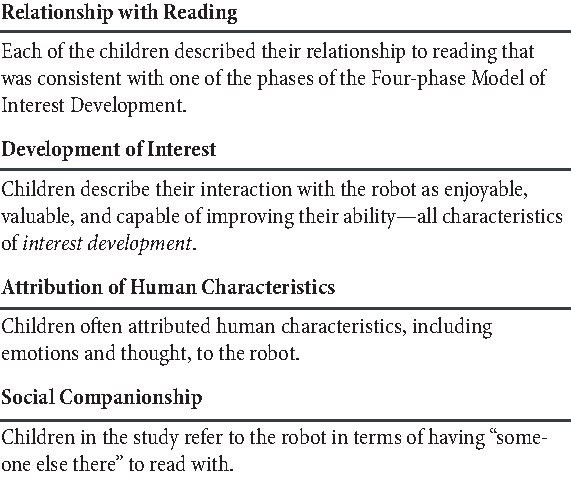
\includegraphics[width=1\columnwidth]{figures/chi17-michaelis-figures-summary.pdf}
	\caption{Summary of each of the themes emerging from our analysis.}
	\label{fig:figure4}
\end{figure}

\subsection{Relationship with Reading}
In recruiting for our study, we initially intended to enroll children with a variety of interest levels in reading. During a short, online, pre-screening questionnaire, we included a question that asked a parent to estimate the amount of time their child spent on reading each week. We believed that this measure would prove useful for inferring a relative interest level but realized soon after we began our visits that this estimate was often not very accurate. Thus, we chose not to make any recruitment decisions based on pre-screening. We instead used pre-interview descriptions of the child's view and habits towards reading to identify what phase of interest in reading they were likely in. While we do not believe that any of our participants are categorized in the first and lowest phase of interest development, \textit{triggered situational interest}, we classified two participants (MC1 and MC2) in phase two, \textit{maintained situational interest}, three (MC3, MC4, and MC5) in phase three, \textit{emerging individual interest}, and three (MC7, MC6, and MC8) in the highest and fourth phase, \textit{well-developed individual interest}. These evaluations were supported by results from each child's FID-RS individual interest survey score. We found that our \textit{phase two} readers had the lowest and second lowest scores (4.5 and 5.4), the \textit{emerging individual interest} readers fell in a range between 5.3 and 5.9, and the \textit{well-develop individual interest} readers had all three of the highest scores that ranged from 6.3 to 7.0 (the scale maximum). Based on information gathered during our pre-interviews, we now turn to describing the children at each level of interest in reading. 

\subsubsection{Phase 4: Well-developed Individual Interest}
Of the three well-developed individual interest readers, one, MC8, had an extreme interest in reading. MC8 reads an exceptional amount (300 or more pages per day), and was described by his parent, P8, as ``off the charts.'' He is such an avid reader that the local bookstore supplies him with ``a lot of advanced readers of books each month'' to have him ``give them an opinion on the books.'' He described having very little need for a reading technology and struggled to find ideas of what one might do, because he felt no need to support improving his reading ability or motivation to read.

Our two other high interest readers, MC6 and MC7, described themselves as having high reading ability, and that they were an ``avid reader,'' and ``always loved to read,'' respectively. While they felt that they were very good readers, they both indicated that they would like to continue to develop their reading ability. To support this development, they both thought a technology might suggest new books for them to read. MC6 also added a desire for a technology that would track their reading and provide some level of motivational support, while MC7 mentioned an interest in reading out loud.

\subsubsection{Phase 3: Emerging Individual Interest}
Our three emerging individual interest readers read between 30 to 60 minutes on an average day and find that they can become engrossed in the right book. However, they often struggle to find new books that interest them and are continually seeking out new material. For example MC4 said, ``I go out and try to find new books but I don't, like, find that many books appealing to me.'' This behavior may be due to being reluctant to invest in reading new books, which leads them to re-read many of the books they already have several times. They value reading as a way to learn, believe that they are ``okay'' readers and would like to ``practice and get better,'' and appreciate ways of being supported in developing their ability. They also recognize a need for some external motivational support, particularly when they do not connect with a book right away (even if it is just a ``nagging mom''). MC3 did not suggest anything he would want a reading technology to do. However, both MC4 and MC5 would like a technology to help them understand and pronounce words while they read and to give them feedback about the book as they read.

\subsubsection{Phase 2: Maintained situational interest}
Both of our maintained situational interest readers described themselves as capable readers. While both said that they only ``like reading a little,'' they reported enjoying reading when they really like a book. However, they reported different amounts of time spent reading; MC1 read 30 minutes a day, because this is the goal her parents sets for her, while MC2 read very little outside of what is required for school. They both felt that reading is something that they should do more of but did not prioritize among other activities. Thus, they did not seek out reading unless required. For MC2, this conflict of feeling that he should read more but not really making the time for it appeared in our interview when describing that it is hard for him to find a book. He said, ``Yeah I am like looking right now. Well I am trying to get time to look for books. Well I mean I have got a lot of time but...,'' indicating that while he feels that he should be looking for an interesting book, he is not actively doing so. Both children mention that tracking their reading with a log has been an effective method of motivation, although MC2 no longer uses any tracking, and both said that logging and tracking would be welcome features in a reading technology. MC1 also added that she would like a technology that would ``Listen to [her] and tell [her] what it thought of the book or what [they] read.'' MC2 indicated that he would like a technology that could support understanding by adding illustrations to depict what was happening in the text. Both of their parents mentioned motivational support as something they would like a technology to offer.

Having established each child's relationship with reading, summarized in Table~\ref{tab:table1}, we will now begin describing themes that emerged from observations of the children interacting with the robot and their post-interviews.


\begin{table}[]
	\centering\footnotesize
	\begin{tabular}{cccc}
		& {\small \textbf{Phase}} & & {\small \textbf{FID-RS}} \\
		{\small \textbf{Participant}} & {\small \textbf{Number}}& {\small \textbf{Phase of Interest}}
		& {\small \textbf{Score}} \\
		\midrule		
		MC1  & 2       & \textit{maintained situational}    & 4.5    \\[0.75ex]
		MC2  & 2       & \textit{maintained situational}    & 5.4    \\[0.75ex]
		MC3  & 3       & \textit{emerging individual}      & 5.4    \\[0.75ex]
		MC4  & 3       & \textit{emerging individual}       & 5.3    \\[0.75ex]
		MC5  & 3       & \textit{emerging individual}       & 5.9    \\[0.75ex]
		MC6  & 4       & \textit{well-developed individual} & 6.7    \\[0.75ex]
		MC7  & 4       & \textit{well-developed individual} & 7.0    \\[0.75ex]
		MC8  & 4       & \textit{well-developed individual} & 6.3   \\[0.75ex]
		\midrule     
	\end{tabular}
	\caption{Phase of interest for main child participants. The FID-RS score is a measure of individual interest in reading. Note that no participants were found to be in phase 1.}
	\label{tab:table1}\normalsize
\end{table}

\subsection{Development of Interest}

Our initial design of the learning companion robot was heavily influenced by interest development theory, and our analysis found that the children in our study describe much of their interaction in terms of the characteristics of interest development: \textit{positive affect} (i.e., enjoyment), \textit{value} for the interaction, and increasing ability or \textit{knowledge} as a result of the interaction. Positive affect was generally mentioned across all participants. All said that they liked something about their interaction with Minnie and described the interaction as ``nice,'' ``fun,'' and ``cool.'' Positive affect was attributed equally across all the interaction features that the children mentioned.
	\begin{quote}
		\textbf{MC5:} I liked how she could recommend books and she commented during the book about different parts.
	\end{quote}
		
Phase 4 children were much less likely than those in phase 2 or 3 to talk about their interaction with the learning companion robot as a helpful or valuable experience. For those in phase 2 and 3, positive affect and value were often attributed to specific aspects of the interaction with the learning companion robot. While these comments were evenly distributed across all the features mentioned, with one exception: tracking reading time and page numbers was only mentioned by half of the families. Both MC2 and MC6 suggest that they ``like'' this feature and it was ``nice,'' and three children across all phases of interest (MC2, MC4, MC6) refer to the robots ability to track their progress as ``helpful.'' For example: 
	% TODO: This last sentence is not clear. Do we meant that this feature was disproportionately mentioned in interviews? Or some participants mentioned it more than others?
	% DONE: Condensed and clarified.  It was the only one that was mentioned by the majority of families, so that stood out.
	\begin{quote}
	\textbf{MC2:} It was helpful because that way if you take a break, he still knows what page you are on.
	\end{quote}
	
We found that only families who refer to this type of tracking as something they would want a technology to do in pre-interviews were the ones who discussed it after interacting with Minnie. Many families had also explained that tracking had been a way of helping to motivate their children, but none said that this feature offered any motivational support. It may be that our method of tracking was not conducive to increased motivation to read, but was rather only a nice and helpful feature to manage the process of reading.
% TODO: We need to clarify the main finding here. Is it that tracking was a generally desirable feature but no one found it to motivate them? Were we really expecting it? If it is one design feature, is it too much to expect that it would increase overall motivation anyway? 

In contrast to children referencing many different features of the robot interaction when describing positive affect and value, only two features were mentioned in reference to improving reading ability. Comments made by Minnie during the reading was thought to be a way to improve reading comprehension. Children felt that Minnie's comments were a way of ``recapping'' or helping them see the story from ``a different perspective.'' Reading out loud was a feature of the interaction that children described as potentially improving their reading skills (e.g., vocabulary and pronunciation).

	\begin{quote}
		 \vspace{2mm}
		 \textbf{R:} You kind of talked about the difference about reading out loud. And that, you asked early if you should read out loud. Umm.. Did you like that experience?
		 		 
		 \textbf{MC4:} It kind of helped with some words, but at the same time, it didn't really help with other words.
		 
		 \textbf{R:} Okay, what do you mean by ``helped''? Helped with what?
		 
		 \textbf{MC4:} Like, helped me, like, pronounce them better.
		  
		 \textbf{R:} Okay. Do you think, so is that, kind of, building...like is that making you better at reading you mean? Or...
		 
		 \textbf{MC4:} Uhh...yeah. 
		 
	\end{quote}

Describing the interaction with Minnie as a way to develop reading ability was almost entirely done by phase 3 readers. Children in phase 2 and phase 4 each only mention improving reading ability once and focus more on liking the learning companion robot and how the interaction was helpful to the process of reading but not necessarily their ability to read. This behavior may indicate that the support provided by Minnie to improve reading ability is a good match for children who feel they are good readers but need a little help with both comprehension and reading skill. When we asked our families about improvements or changes they would make to the learning companion robot, those in phase 2 focused on changing the interaction to better support reading ability, while those in other phases mentioned ways of improving ease of use. 

	\begin{quote}
	 \textbf{P1:} He likes to read with someone.
	 
	 \textbf{MC1:} Cause he doesn't know if he's gonna get the word right.
	 
	 \textbf{R:} Ohh, okay, so . . . If you were mispronouncing a word or like said something wrong would you want a robot to tell you that, or would you rather the robot just kind of like let it go?
%	 TODO: The first sentence of the quote seems to be missing a word. Should we paraphrase? 
% DONE: Better? I wanted to capture that my sugggestion was rephrasing what they said. My fix added lines though, maybe we paraphrase to save on length? 
	 
	 \textbf{P1:} ((shakes head ``yes''))
	 
	 \textbf{OC1:} [She should] tell me that. 
	 
	 \textbf{R:} ((to MC1)) Would you wanna know?
	 
	 \textbf{MC1:} Yeah.
	 
	 \textbf{R:} Yeah, ok. Would that be like, when would you wanna know that? Would it be at the end of the whole thing or would it be right away while your reading?
	 
	 \textbf{MC1:} Right away. Like if it was a chapter book, at the end the chapter [it] would tell you all the words that you got wrong and [you] had to say them.
	\end{quote}

For our assessment of how interest may be developed as a result of the interaction, we consider how well the learning companion robot might help children at differing phases of interest in reading develop interest. We find that Minnie, as designed, may be best suited for those in an emerging individual phase of interest (phase 3). These children expressed experiencing all three characteristics of interest development---positive affect, value, and ability development---as a result of their interaction with Minnie, and support across all these areas is important for developing interest at this phase. Minnie may also be appropriate for our maintained situational interest (phase 2) and well-developed individual interest (phase 4) participants, although its benefits for those at extreme levels of interest (i.e., MC8) would likely be limited. Their interest in reading did seem to be triggered from their enjoyment of the interaction and the value they found in working with Minnie---both important factors in developing interest in a domain. However, some modifications to improve the learning companion's capacity for supporting the improvement of reading ability at higher and lower levels are needed. Suggestions for future improvement from our families indicate that these modifications might include ``chapter summaries'' or ``comprehension questions'' for our phase 2 readers; and the option to read silently or connect ``outside of the book to other places'' for phase 4 readers.
% TODO: What does "scanning for Minnie's comments mean?
% DONE: Yeah, that was confusing.  I just cut it.  The imporant ideas was that they didn't like reading outloud as much.

\subsection{Attribution of Human Characteristics}

In order to best promote reading engagement and interest, we deliberately designed our learning companion robot to act in a social way. One important indicator that this goal was achieved came from our participants' attribution of several human characteristics to Minnie. The families described the robot as being able to ``look,'' ``listen,'' ``talk,'' and ``understand'' as well as having personality characteristics such as being ``jolly,'' ``pleasant,'' and ``funny.'' They also attributed thoughts and feelings to the robot such as feeling ``happy,'' making ``connections'' to what you were reading, appearing to have ``liked the book'', and seeming to ``[have] something to say.'' When asked why they got this impression, many referenced the feedback and comments as well as the physical movements made by the robot. 

Notions about Minnie's feelings and personality came from both physical and software design. Specifically, Minnie's physical shape (e.g., enlarged rounded head and large eyes) seemed to influence perception of her personality, and it's speech capabilities that were tied to the specific context seemed to give the appearance of thoughts and feelings. 

One feature of the learning companion robot design that had a significant impact on this impression of human characteristics appeared to be the continuous face tracking during the interaction. Not only was the robot designed to orient its head toward each face detected but to also include intervals of randomized movements in other directions. MC6 noted that it felt like the robot was ``looking'' at her, and while MC1 worked with Minnie, her sibling, sitting near them, noted that Minnie would point her head directly at each of them and other places in the room.
% TODO: The "was staring at you" comment is a bit confusing. Is it staring such that it's uncomfortable? And is "you" MC6?

% DONE: Changed the quote to something she had said a second before.  This ought to make it clear that it wansn't in a creepy way, and that it was looking at her.

	 \begin{quote}
	 	 \textbf{OC1:} It like looked around the room and saw stuff, and it was looking at me and MC1 a lot.
	 \end{quote}
	
Feeling that Minnie could understand was often attributed to what the learning companion robot would say. Families felt that Minnie ``knew your name,'' because she would use the child's name when saying hello. They also saw her comments during the reading phase to be an indication that she could comprehend the story.

	\begin{quote}
		\textbf{MC6:} She talked about the whole thing you've read and the chapter, cause after I read how someone in one book put up a sign on their door she asked like `Oh I wonder why was there a sign on the door?'
	\end{quote} 

Based on prior work in human-robot interaction, we did anticipate the attribution of human characteristic to the robot.
% TODO: Can we include a citation to the work we are referring to?
% NOTE: This is a big question I have.  Should we include this in the background.  I don't want to introduce new lit this late in the paper, but I worry about adding things that would be construed as design guidelines since we are locked in at 8.  I have three good citations for this that I found last night, they are commented out in the background section. Thoughts?

Based on guidelines from this literature for designing engaging social robots, we intentionally integrated aspects of social behavior in order to further our goals in designing the robot as a learning companion. While we thought of social interaction as a way to improve overall engagement with the robot, we were surprised to find that the social interaction tapped into a desire for social companionship while reading.

\subsection{Social Companionship}

The combination of the social behavior of the robot with the children's desire to socially engage while reading produced an effect that we describe as \textit{social companionship}. We did not expect the children in the study to express a desire to socially engage while reading, as it is commonly characterized and pursued as an individual activity. However, the idea of social companionship was touched on by most families, with the exception of MC3 and MC8, during our interviews. For the families who spoke about reading \textit{with} someone, a lack of social companionship was cited as a reason that reading could be boring, and reading together was a habit in which many of our families currently engaged. Since Minnie was designed to behave socially, this behavior seemed to help children find social companionship while they read with it. 
% TODO: I believe that this is the most surprising and interesting finding of the study. Can we elevate this to emphasize? We can further emphasize it in discussion and repeat in conclusion. You already have this in the title of the paper, but the reader doesn't come to it until page 9, so it's somewhat buried in there. Can you see ways of bringing this out?

Not only was social companionship positively discussed by almost all of our families during our interviews, but it also appeared to be beneficial across all phases of interest. Both of our phase 2 readers felt that it helped them engage with the reading activity. MC1 had complained that reading is usually boring, but she said Minnie ``encouraged me'' and reading with it was enjoyable because there was someone else there.
	
	\begin{quote}
		\textbf{R:} Did you enjoy working with Minnie?
		
		\textbf{MC1:} ((shake of head ``yes''))
		
		\textbf{R:} What was nice about it?
		
		\textbf{MC1:} ((pauses to think)) I liked the company?
		
		\textbf{R:} Ok, tell me a little about that, what do you mean?
		
		\textbf{MC1:} ((pauses to think)) I don't know. I usually read alone so it was like different.
	\end{quote}

Our other phase 2 reader, MC2, also seemed to find having Minnie there as a social companion while reading to stimulate his motivation to read.  
  
	 \begin{quote}
	   \textbf{MC2:} Because I mean she helps, it is pretty much like having someone there helping you read. So like if I am home alone, I can have it sit out and I can, it can help me with my stuff while I am reading. 
	   
	   \textbf{R:} So, I will come back and I wonder then, so you said a lot of time with reading, you don't really have time for it. Do you think Minnie would make you feel, would you make more time? 
	   
	   \textbf{MC2:} Yes. 
 	\end{quote}
 
The social companionship of reading with Minnie also seemed to be a positive experience for our phase 3 and 4 readers as well, although it took different forms; MC4 liked that reading with Minnie felt like reading to someone younger.
 
 \begin{quote}
 	 \textbf{MC4:} It was a fun change. 
 	 
 	 \textbf{R:} Okay. How so? What do you mean by that?
 	 
 	 \textbf{MC4:} Umm like I found it, like, that... my, the voice in my head that I use when I'm reading to myself sounds different than when I read out loud... It felt like I was reading to a little kid. And, like, helping them understand some stuff.
 	 \end{quote}
 	 
MC5 related the experience to the positive feelings they had while reading with their family.

	\begin{quote}
		
		\textbf{R:} What did you like about it, what was nice?
		 
		 \textbf{MC5:} Um, like the. . . It felt like it was another person listening and like I could communicate with her.
%		 TODO: ...the [way] it...?
% 		DONE: Just stammering at the beginning.  Should I cut that?
		 
		 \textbf{R:} I see. Ok. And I know you said like with your family you guys sort of do that. Did you get that same sort of sense of like you and Minnie were sort of like reading together and sort of sharing the book?
		 
		 \textbf{MC5:} Yeah.
	\end{quote}

MC6 found that the social companionship led to better reading.

	\begin{quote} 	
		 \textbf{MC6:} It . . .  kind of just listened to you instead of just you reading by yourself.
		 
		 \textbf{R:} How did the listening to you, how did that make your reading different?
		 
		 \textbf{MC6} Um, maybe because. . . ((pause of 2 seconds)) cause you actually tried to do really good. Instead of just like.
%		 TODO: Should "2 seconds" be in (( ))?
% DONE: Yup, and I added some words to make it more clear
		 
		 \textbf{R:} So, you maybe did a better job of reading because Minnie was listening to you, you said?
		 
		 \textbf{MC6:} Mhmm [yes]. 
 \end{quote}
 
 Finally, MC7 found that through the comments while reading, Minnie took on a social companion role similar to MC7's friends who read the same books as her.
 
	 \begin{quote}
	 	  \textbf{MC7:} Umm well, like, at the end of the, like, end of the thing when you scanned, like, she would, like, kind of comprehend what you were reading it seemed like. And she would, like, make connections just like a friend would do. 
	 	  
	 \end{quote}
 
As discussed above, the social aspects of our learning companion robot were not intended to allow Minnie to provide social companionship. We found, however, that this experience was common for our participants and was an effect across all phases of interest. There is also evidence that the added social companionship of reading with our learning companion robot addresses each of the major areas of interest development: increases in positive affect, value, and knowledge and skills in the domain.  

\section{DISCUSSION}
The four themes that emerged from our Grounded Theory analysis suggest two major design implications: providing support for interest development across all phases of interest, and intentially designing for social companionship.  The findings may also be applied to other academic domains such as math or science education, and could prove valuable as design considerations for pedagogical agents in other educational technologies.  In this section we will discuss these design implications, as well as limitations to the study and potential future work.

\subsection{Supporting Interest Development}
While generating positive affect for a task or area of study is important, reseachers also note that supporting students to find value for a domain (e.g. reading) and improving knowledge and ability in the task are also critical to interest development.  As we looked for emerging themes from our data, positive affect, value, and knowledge building were often referenced by families.  We found that interacting with Minnie was generally well liked by all of the families that we visited across all phases of interest.  This positive experience was attributed to numerous design elements of the learning companion robot.  These include 


\subsection{Limitations}

\section{CONCLUSION}
Our use of the technology as a probe into the reading habits of young readers help us understand more about a learning companion...


\section{Acknowledgments}
Removed for blind review.

\balance{}

\bibliographystyle{SIGCHI-Reference-Format}
\bibliography{chi17-michaelis}

\end{document}
